% This file was created with tikzplotlib v0.10.1.
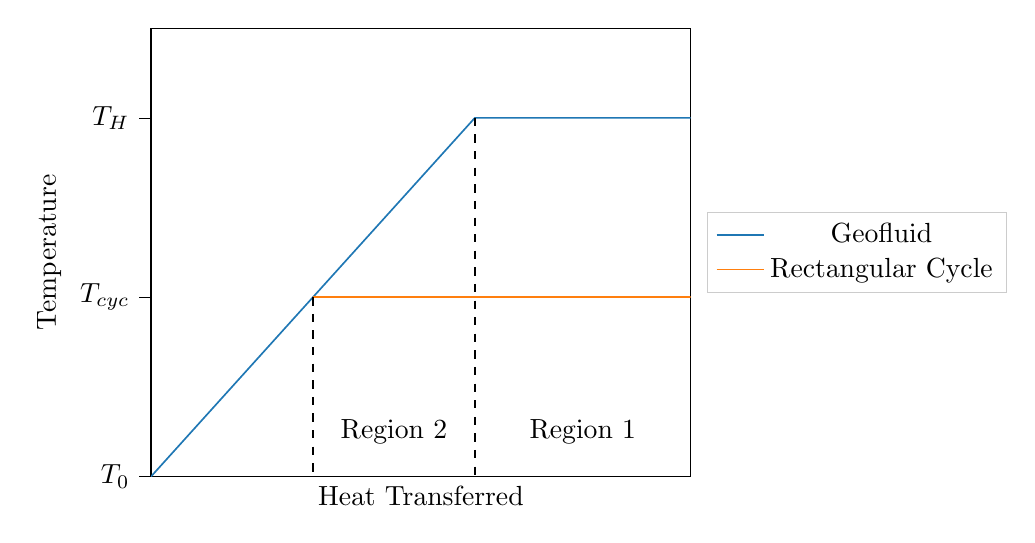
\begin{tikzpicture}

\definecolor{darkgray176}{RGB}{176,176,176}
\definecolor{darkorange25512714}{RGB}{255,127,14}
\definecolor{lightgray204}{RGB}{204,204,204}
\definecolor{steelblue31119180}{RGB}{31,119,180}

\begin{axis}[
legend style={
  fill opacity=0.8,
  draw opacity=1,
  text opacity=1,
  at={(1.03,0.5)},
  anchor=west,
  draw=lightgray204
},
tick align=outside,
tick pos=left,
x grid style={darkgray176},
xlabel={Heat Transferred},
xmin=0, xmax=10,
xtick style={color=black},
y grid style={darkgray176},
ylabel={Temperature},
ymin=0, ymax=10,
ytick style={color=black},
ytick={0,4,8},
yticklabels={
  \(\displaystyle {T_0}\),
  \(\displaystyle {T_{cyc}}\),
  \(\displaystyle {T_H}\)
},
xmajorticks=false
]
\addplot [semithick, steelblue31119180]
coordinates {
            (10, 8)
            (6, 8)
            (0, 0)
                };
\addlegendentry{Geofluid}
\addplot [semithick, darkorange25512714]
coordinates {
            (3, 4)
            (10, 4)
                };
\addlegendentry{Rectangular Cycle}
\addplot [semithick, black, dashed]
coordinates {
            (3, 4)
            (3, 0)
                };
\addplot [semithick, black, dashed]
coordinates {
            (6, 8)
            (6, 0)
                };

\node at (axis cs:8,0.5) [anchor=south] {Region 1};
\node at (axis cs:4.5,0.5) [anchor=south] {Region 2};
                
\end{axis}

\end{tikzpicture}
